\documentclass[smaller, aspectratio=169]{beamer}

\usepackage{silence}
\WarningFilter{remreset}{The remreset package is obsolete}
\usetheme{Boadilla}
\usecolortheme{rose}
\usepackage{slides_preamble}
\usepackage[autopunct=true, hyperref=true, doi=false, isbn=false, natbib=true, 
url=false, eprint=false, style=chicago-authordate]{biblatex} 
\addbibresource{risk_bibliography.bib}
\setbeamercovered{invisible}

\let\emph\relax 
\DeclareTextFontCommand{\emph}{\color{DarkGreen} \bfseries}

\title[]{Identification Robust Inference for Risk Prices in Structural Stochastic Volatility Models} 
\author[Cheng, Renault, and Sangrey]{Xu Cheng \inst{1} \and Eric Renault \inst{2} \and Paul Sangrey \inst{1}}
\institute[]{\inst{1} University of Pennsylvania \and \inst{2} University of Warwick}
\date[]{March 25, 2019}

\newcommand*{\rkappa}{\textcolor{red}{\kappa}}
\newcommand*{\rpi}{\textcolor{red}{\pi}}

\begin{document}

\begin{frame}[plain, noframenumbering]
	\maketitle
\end{frame}

 
\section{Introduction}

\begin{frame}[c]{Introduction}

  \begin{itemize}
    \item How do investors trade off risk and return? \textcites{sharpe1964capital}.
      \medskip
%
    \item The capital asst pricing model (CAPM) gives a static trade-off.
      \medskip
%
    \item In practice, volatility varies over time.
      \medskip
%
    \item Modern asset pricing models often include an additional channel, e.g., \textcites{chang2013market, dewbecker2017price}.
      \smallskip
%
    \begin{itemize}
      \item Investors care directly about changes in volatility.
    \end{itemize}
  \end{itemize}
\end{frame}


\begin{frame}[c]{Volatility Affects Expected Returns Through Two Channels}

  \begin{enumerate}
    \item Investors' willingness to tolerate high-volatility to get high expected returns.
        \medskip
      \begin{itemize}
          \item This measured by the \emph{market return risk price} --- $\rkappa$.
      \end{itemize}
%
      \bigskip
%
        \item Investors' direct aversion to changes in future volatility.
        \medskip
      \begin{itemize}
          \item This is measured by the \emph{volatility risk price} --- $\rpi$.
      \end{itemize}
  \end{enumerate}
%
      \bigskip \pause
%
  \begin{itemize}
    \item \Textcite{han2018leverage} disentangle the two channels when the leverage effect is \emph{large}. 
%
        \medskip \pause
%
    \item However, the leverage effect is \emph{small} and hard to estimate, \parencites{aitsahalia2013leverage, bandi2012timevarying}.
  \end{itemize}

  \pause
  \bigskip

  \begin{block}{Problem}
      $\rpi$ is \emph{weakly-identified}. We develop robust methods to create \emph{uniformly-valid confidence sets} regardless of the identification strength.
  \end{block}
  
\end{frame}

\begin{frame}[c]{Literature Review}

    \emph{Analyzing the Relationship between Risk and Return:} 

    \begin{itemize}
        \item  The empirical literature estimating  $\rkappa$ is inconclusive, \parencite{lettau2010measuring}. 
%
        \item \Textcites{bollerslev1988capital, harvey1989timevarying, ghysels2005there} find a positive estimate.
% 
        \item \Textcites{campbell1987stock, breen1989economic, brandt2004relationship} find a negative one.
%
        \item \Textcites{christoffersen2013capturing, feunou2014risk, dewbecker2017price} focus on the theory and contain both risk factors.
    \end{itemize}
    
    \pause

    \emph{Analyzing Weak Identification:}

    \begin{itemize}
        \item \Textcites{staiger1997instrumental, mavroeidis2014empirical, andrews2015maximum} examine various empirical applications in linear IV and nonlinear structural models.
%
        \item \Textcite{moreira2003conditional} introduces the conditional inference approach we use, \textcite{kleibergen2005testing} extends it to nonlinear GMM, and \textcite{andrews2016conditional} cover infinite-dimensional nuisance parameters.
\end{itemize}

\end{frame}


\begin{frame}[c]{Plan for the Talk}
  \begin{enumerate}
%
    \item The model.
      \bigskip
%
    \item Asymptotic results for the reduced-form and structural parameters.
      \bigskip
%
    \item Confidential inference algorithm for minimum distance estimation and accompanying theory. 
      \bigskip
%
    \item Simulation results. 
      \bigskip
%
    \item Empirical results using data on the S\&P 500.
%
  \end{enumerate}
\end{frame}

\section{Theory}

\begin{frame}[c]{The Model}

    \begin{tabularx}{\textwidth}{X | X}
        \multicolumn{2}{c}{Asset Pricing Equation:} \\
        \toprule 
        \multicolumn{2}{l}{} \\
%
        \multicolumn{2}{l}{\emph{--} $\displaystyle P_t = \E\left[M_{t, t+1} \exp(-r_f) P_{t+1} \mvert \F_{t} \right]$.} \\
%
        \multicolumn{2}{l}{\emph{--} $\displaystyle M_{t, t+1}(\rpi, \rkappa) = \exp\left(m_0 + m_1 \sigma^2_t - \rpi \sigma^2_{t+1} - \rkappa r_{t+1}\right)$.} \\ 
        \multicolumn{2}{l}{} \\
%
        \toprule
        \multicolumn{2}{c}{\only<2->{Reduced-Form Model}} \\ 
        \toprule 
%
        \only<2->{$\sigma^2_{t+1}$ follows a conditional autoregressive gamma process:} & \only<3>{$r_{t+1}$ follows a conditionally Gaussian process:} \\
%
        \only<2->{\\[-\normalbaselineskip] \midrule} \\
%
        \only<2->{$\displaystyle \E\left[\exp(-x \sigma^2_{t+1}) \mvert \F_t\right] = \exp(-A(x) \sigma^2_{t} - B(x)) $.} & 
        \only<3>{$\displaystyle \E\left[\exp(-x r_{t+1} \mvert \F_t, \sigma^2_{t+1} \right]$}  \\ 
        & \only<3>{\qquad $ \displaystyle = \exp(-C(x) \sigma^2_{t+1} - D(x) \sigma^2_t - E(x))$.} \\ 
%
        \only<2->{$\displaystyle A(x) \coloneqq \frac{\rho x}{1 + c x}$.} & \only<3>{$\displaystyle C(x) \coloneqq \psi x - \frac{1-\phi^2}{2} x^2 $.} \\
%
        \only<2->{$\displaystyle B(x) \coloneqq \delta \log(1 + c x)$.} & \only<3>{$\displaystyle D(x) \coloneqq \beta x$.} \\
%
                                                                           &  \only<3>{$\displaystyle E(x) \coloneqq \gamma x$.}  \\
        \bottomrule
%
    \end{tabularx}
\end{frame}



\begin{frame}[c]{Identification}

  \begin{minipage}{.49\textwidth}
    \centering
    \emph{The Link Functions}
%
    \begin{enumerate}
      \item $\displaystyle \gamma = B(\rpi + C(\rkappa -1)) - B(\rpi + C(\rkappa))$. 
%
      \item $\displaystyle \beta = A(\rpi + C(\rkappa -1)) - A(\rpi + C(\rkappa))$. 
%
      \item $\displaystyle \psi = \frac{\phi}{\sqrt{2 c}} - \frac{1-\phi^2}{2} + (1 -\phi^2) \rkappa$.
    \end{enumerate}
  \end{minipage}%
%
  \hfill
%
  \pause
%
  \begin{minipage}{.49\textwidth}
    \centering
    \emph{Identification Problem}
    \begin{enumerate}
        \item $\rpi$ is not identified if $C(\rkappa - 1) = C(\rkappa)$.
        \item $C(\rkappa - 1) - C(\rkappa) $
        \item[=] $\psi - \frac{1 - \phi^2}{2} (2 \rkappa -1 )$
        \item[=] $\frac{\phi}{\sqrt{2 c}}$.
    \end{enumerate}
  \end{minipage}

\end{frame}


\begin{frame}[c]{Estimating the Reduced-Form Parameters}


  \begin{enumerate}
  \item We estimate $\omega_1 \coloneqq \begin{pmatrix} \rho & c & \delta \end{pmatrix}'$ using two-step GMM
%
      \begin{equation*}
        \widehat{\omega}_{1} \coloneqq \underset{\omega_{1}\in O_{1}}{\arg \min}\left(T^{-1}\sum_{t = 1}^{T}h_{t}(\omega_{1})\right)^{\prime}\widehat{V}_{1}\left(T^{-1}\sum_{t=1}^{T}h_{t}(\omega_{1})\right), 
      \end{equation*}
      %
      where $\widehat{V}_{1}$ consistently estimates $V_{1} \coloneqq \sum_{m=-\infty}^{\infty}\Cov[h_{t}(\omega_{10}), h_{t+m}(\omega_{10})].$
%
      \bigskip
%
  \item We estimate $\omega_{2} = \begin{pmatrix} \gamma & \beta & \psi \end{pmatrix}'$ using generalized least squares: 
%
      \begin{equation*}
        \widehat{\omega}_{2} \coloneqq \left( \sum_{t=1}^{T}x_{t}x_{t}^{\prime}\right)^{-1}\sum_{t=1}^{T}x_{t}y_{t}, \text{ where } 
      %
x_{t} \coloneqq \frac{1}{\sigma_{t+1}} \begin{pmatrix} 1 & \sigma_{t}^{2} & \sigma_{t+1}^{2} \end{pmatrix}'  \text{ and } y_{t} \coloneqq \frac{r_{t+1}}{\sigma_{t+1}}. 
      \end{equation*}
%
      \bigskip
%
    \item We estimate $\omega_{3} \coloneqq 1 - \phi^2$ by the sample variance estimator:
%
      \begin{equation*}
        \widehat{\omega}_{3} \coloneqq T^{-1}\sum_{t=1}^{T}\left(y_{t}-\widehat{y}_{t}\right)^{2}, \text{ where } \widehat{y}_{t} = x_{t}^{\prime}\widehat{\omega}_{2}. 
      \end{equation*}
      
  \end{enumerate}
      

\end{frame}

\begin{frame}[c]{Assumptions for any $\theta$, $\omega$ close to its true value, and $ 0 < C < \infty$.}

  \begin{block}{Assumption R}
    \label{assump:R}
%    
    \begin{enumerate}
      \item Let $T^{-1}\sum_{t=1}^{T}(h_{t}(\omega_{1})-\E[ h_{t}(\omega_{1}))\rightarrow_{p}0$ and $T^{-1}\sum_{t=1}^{T}(H_{t}(\omega_{1})-\E[H_{t}(\omega_{1})])\rightarrow_{p}0$, and $\E[H_{t}(\omega_{1})]$ be continuous in $\omega_{1}$; all holding uniformly.
%
      \item Let $T^{-1}\sum_{t=1}^{T}(x_{t}x_{t}^{\prime}-\E[ x_{t}x_{t}^{\prime}{])\rightarrow}_{p}0.$
%
      % \item $V^{-1/2} (T^{-1/2}\left(\sum_{t=1}^{T}f_{t}(\omega_{0})-\E[f_{t}(\omega_{0})]\right) \rightarrow_{d} \N(0, \I)$ and $\widehat{V} -V\rightarrow_{p}0.$
      \item Assume the appropriately standardized moment conditions converge to $\N(0, \I)$.
%
  \item Let $V$, $\E[H_{t}\left(\omega_{1, 0}\right)^{\prime}H_{t}\left(\omega_{1, 0}\right) ])$, and $\E[x_{t}x_{t}^{\prime}], \E[ z_{t}z_{t}^{\prime}]$,  have uniformly-bounded eigenvalues where $z_{t} \coloneqq \begin{pmatrix} 1 & \sigma_{t}^{2} & \sigma_{t}^{4} \end{pmatrix}'$.
%
    \end{enumerate}
  \end{block}
  
  \vfill

  \begin{block}{Assumption S}
%
    \begin{enumerate}
      \item Assume the link function --- $g(\theta, \omega)$ --- is partially differentiable in $\omega$, with derivative --- $G(\theta, \omega)$ --- that is Lipschitz in both arguments. 
    %
      \item Assume $(G(\theta, \omega)^{\prime}G(\theta, \omega))$ has uniformly-bounded eigenvalues.
    \end{enumerate}

  \end{block}

\end{frame}


\begin{frame}[c]{Definitions}

    \begin{block}{Criterion}
        \begin{equation*}
          QLR(\theta_{0}) \coloneqq T \widehat{g} (\theta_{0})^{\prime}\widehat{\Sigma} (\theta_{0}, \theta_{0})^{-1}\widehat{g}(\theta_{0})-\underset{\theta \in \Theta}{\min}T\widehat{g}(\theta)^{\prime}\widehat{\Sigma} (\theta, \theta)^{-1}\widehat{g}(\theta),  
        \end{equation*}
        %
        \quad where $\widehat{\Sigma}\left(\theta_{1}, \theta_{2}\right) = \widehat{G}(\theta_{1})\widehat{\Omega}\widehat{G}(\theta_{2})^{\prime}$ and $\widehat{\Omega}$ consistently estimates the first-stage covariance.
    \end{block}
 
    \vfill
    \pause
%
    \begin{block}{Residual Process}
    %
        \begin{equation*}
          \widehat{r}(\theta) \coloneqq \widehat{g}(\theta)-\widehat{\Sigma}(\theta, \theta_{0})\widehat{\Sigma}(\theta_{0}, \theta_{0})^{-1}\widehat{g} (\theta_{0}). 
        \end{equation*}
    %
    \end{block}

\end{frame}

\begin{frame}[c]{Construct the Critical Value through Projection}

Obtain the $1-\alpha $ conditional quantile of the QLR statistic, denoted $c_{1-\alpha }(r,\theta_{0})$: 
\bigskip

\begin{enumerate}
    \item Take $B$ draws $\eta_{b}^{\ast} \overset{i.i.d.}{\sim} \N(0,\widehat{\Sigma}(\theta_{0},\theta_{0}))$. 
%
        \medskip
%
    \item Produce a simulated process, 
%
        \begin{equation*}
            g_{b}^{\ast}(\theta) \coloneqq \widehat{r}(\theta) + \widehat{\Sigma}(\theta, \theta_{0}) \widehat{\Sigma}(\theta_{0},\theta_{0})^{-1}\eta_{b}^{\ast},
        \end{equation*}
%
        and simulated statistic,
%
        \begin{equation*}
            QLR_{b}^{\ast}(\theta_{0}) \coloneqq T\widehat{g}(\theta_{0})^{\prime}\widehat{\Sigma}(\theta_{0},\theta_{0})^{-1}\widehat{g}(\theta_{0})-\underset{\theta \in \rpi}{\min}Tg_{b}^{\ast}(\theta)^{\prime}\widehat{\Sigma} (\theta ,\theta)^{-1}g_{b}^{\ast}(\theta).
        \end{equation*}
%
        \item  Let $b_{0}=\lceil (1-\alpha) B \rceil$. 
        \medskip
%
        \item Then $c_{1 - \alpha}(r, \theta_{0})$ is the $b_{0}^{th}$-smallest element in $\lbrace QLR_{b}^{\ast} \rbrace$.
    \end{enumerate}

\end{frame}

\begin{frame}[c]{The Algorithm}
    \bigskip
  \begin{enumerate}
    \item Estimate the reduced-form parameter $\widehat{\omega} \coloneqq \left(\widehat{\omega}_{1}, \widehat{\omega}_{2}, \widehat{\omega}_{3}\right)'$, following the estimators defined above.
      \bigskip
%
    \item Estimate $\widehat{\omega}$'s asymptotic covariance, $\widehat{\Omega}$, using a sandwich-form estimator.
      \bigskip
  
    \item For $\theta_{0}\in \Theta$, 
          \medskip
%
    \begin{enumerate}
      \item Construct the QLR statistic $QLR(\theta_{0})$ using $g(\theta, \omega), $ $G(\theta, \omega), $ $\widehat{\omega}, $ and $\widehat{\Omega}.$
          \medskip
%
      \item Compute the residual process $\widehat{r}(\theta)$.
          \medskip
  
      \item Given $\widehat{r}(\theta), $ compute its critical value $c_{1-\alpha}(r, \theta_{0})$ as done on the previous slide.
%
    \end{enumerate}
      \bigskip
%
  \item Repeat these steps for different $\theta_{0}$. Collect the not rejected $\theta_{0}$ to form a nominal level $1-\alpha $ confidence set: 
%
    \begin{equation*}
      CS_{T} = \left\lbrace \theta_{0} \mvert QLR_{T}(\theta_{0})\leq c_{1-\alpha}(r, \theta_{0}. \right\rbrace
    \end{equation*}
  \end{enumerate}

\begin{theorem}
  \label{Lemma CS}
  Let Assumptions R and S hold. Then 
%
    $\displaystyle \underset{T\rightarrow \infty}{\lim \inf}\underset{P\in \mathcal{P}}{\inf}\Pr \left( \theta_{0}\in CS_{T}\right) \geq 1-\alpha$ .
\end{theorem}

\end{frame}

\section{Simulations}


\begin{frame}[c]{Simualtion}
    \begin{table}[htb]
     
     \centering
     \caption{Simulation Set-up}
     \label{tbl:simulationParameters}
     
     \begin{tabularx}{.6\textwidth}{X X c X X}
    
      \toprule
      \multicolumn{5}{c}{Parameter Values used by \textcite{han2018leverage}} \\
      \midrule
      $\delta$ & $\rho$ & $c$ & $\rpi$ & $\rkappa$ \\
      \midrule
      0.6475  & 0.50  & \num[scientific-notation=true]{.00394128} & -10 & 1.7680 \\
      \bottomrule
    %
     \end{tabularx}
    
    \end{table}



    \begin{table}[htb]
     
      \centering
      \caption{Finite-Sample Size of the Standard and Proposed Tests}
      \label{tbl:test_performance}
    
     \sisetup{
      round-mode=places,
      round-precision=2,
     }
     
     \begin{tabularx}{.6\textwidth}{X | S >{{\cellcolor{DarkGreen!20}}} S | S >{{\cellcolor{DarkGreen!20}}} S}
    %
      \toprule
      & {Standard} & {\emph{Proposed}} & {Standard} & {\emph{Proposed}} \\
      
      \midrule
      $\phi$ & \multicolumn{2}{c}{$T$ = 2,000} & \multicolumn{2}{c}{$T$ = 10,000} \\
      \midrule
      -0.01  & 2.4   & 5.2  & 1.7 & 5.6   \\
      -0.10  & 3.3   & 6.7  & 2.6 & 6.2   \\
      -0.40  & 3.3   & 5.3  & 3.4 & 4.9   \\
      \bottomrule
    
     \end{tabularx}
    
    \end{table}

\end{frame}


\section{Data and Empirical Results}


\begin{frame}[c]{Data}
    \begin{itemize}
        \item Use data from January 2003 -- September 2017  from on SPY, which is an ETF tracking the S\&P 500.
            \bigskip
%
        \item Use the daily return as $r_{t+1}$.
            \bigskip
%
        \item Use \textcite{sangrey2018jumps} to compute the total volatility, and use that as $\sigma^2_{t+1}$
            \bigskip
%
        \item We use the S\&P 500 because we want a proxy for the market. We do not want the risk to be diversifiable.
    \end{itemize}
\end{frame}

\begin{frame}[c]{S\&P 500 Volatility and Log-Return}

    \begin{figure}[htb]
    
        \begin{subfigure}[t]{.54\textwidth}
            \centering
            Time Series

            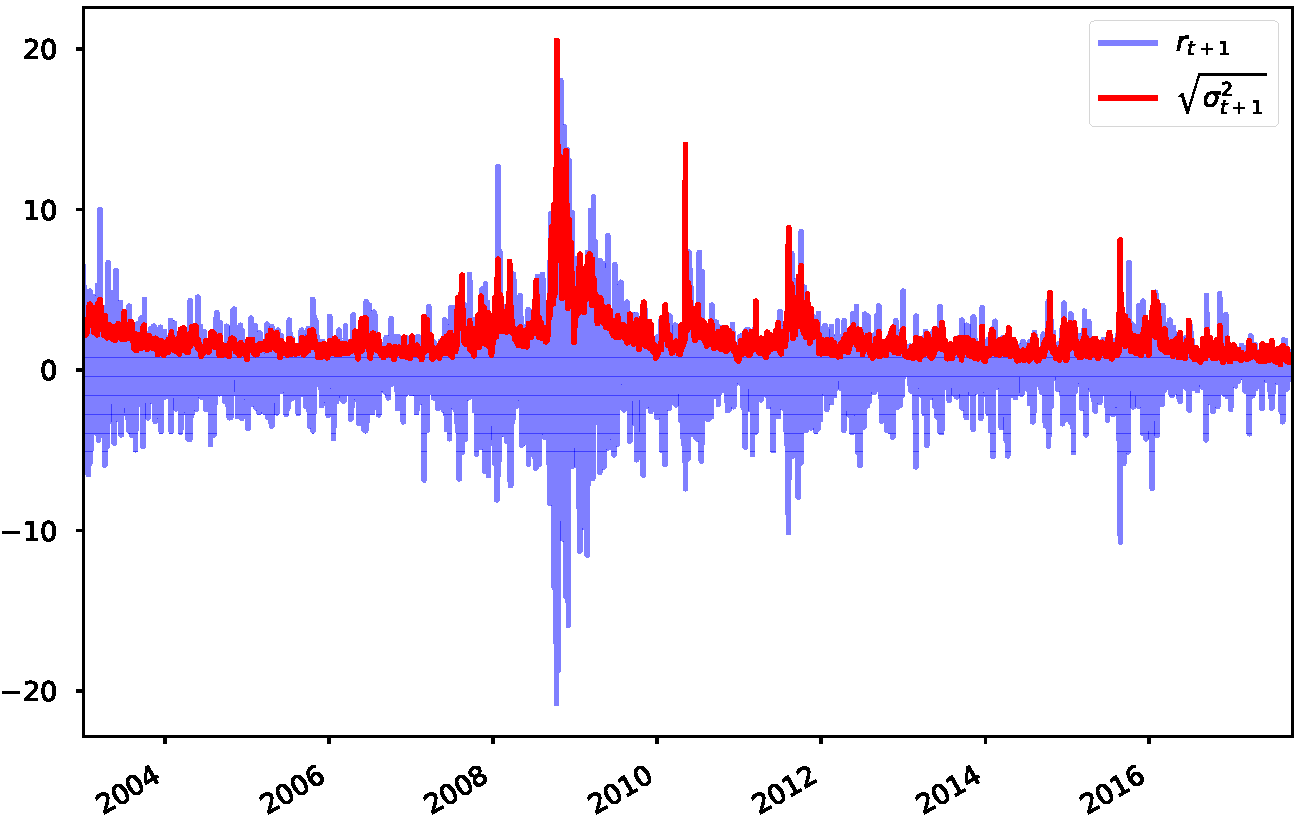
\includegraphics[width=\textwidth, height=.6\textwidth]{time_series.pdf}
        \end{subfigure}%
    %
        \hfill
    %
        \begin{subfigure}[t]{.44\textwidth}
            \centering
            Joint Distribution

            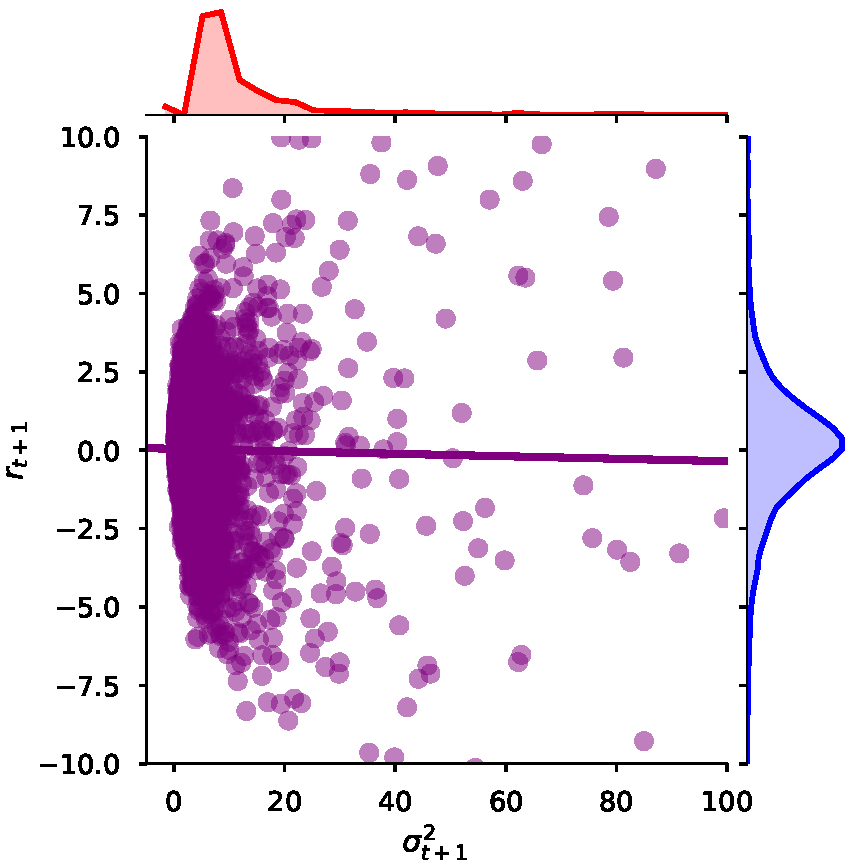
\includegraphics[width=\textwidth, height=.73\textwidth]{joint_dist.pdf}
        \end{subfigure}
    \end{figure}

\end{frame}

\begin{frame}[c]{Summary Statistics}
    \begin{table}[htb]
    
      \centering
      \label{tbl:summary_stats}
    
    
      \sisetup{
       table-align-text-pre     =   false,
       table-align-text-post    =   false,
       round-mode=places, 
       round-precision          =   2,
       scientific-notation      =   false,
       table-space-text-pre     =   \lbrack,
       table-space-text-post    =   \rbrack,
      }
    
        \begin{tabularx}{.5\textwidth}{X | S S}
            \toprule
            & {$r_{t+1}$} & {$\sigma^2_{t+1}$} \\
            \midrule
            Mean & 0.023421 & 5.621287 \\
            \rowcolor{DarkGreen!20}
            Standard Deviation & 2.350165 & 14.458446\\
            Skewness & -0.312 & 12.209 \\
            \rowcolor{DarkGreen!20}
            Kurtosis & 10.055 & 240.401 \\
            Correlation & \multicolumn{2}{c}{\num{-0.024379}} \\
            \bottomrule
        \end{tabularx}
    
    \end{table}

\end{frame}

\begin{frame}[c]{Parameter Estimates}

    \begin{minipage}{.49\textwidth}
        \begin{table}[htb]
            \centering
            Volatility Paramters 
        
            \bigskip
            \sisetup{
                detect-mode,
                tight-spacing           = true,
                group-digits            = false,
                input-symbols           = {(}{)},
                input-open-uncertainty  = ,
                input-close-uncertainty = ,
                round-mode              = places,
                scientific-notation = false,
                round-precision         = 2,
                table-align-text-pre    = false,
                table-align-text-post   = false,
                table-alignment         = center,
            }
        
            \begin{tabularx}{\textwidth}{X | S >{{(}} S[table-space-text-pre={(}] <{{,\,}}
              S[table-space-text-pre={\hspace{-1.5cm}}] <{{)}}}
        %
            \toprule
            & {Point Estimate} & \multicolumn{2}{c}{ 95 \% Confidence Interval} \\
            \midrule
            $c$     & 6.0678 & 3.47006  & 10.6103 \\
            \rowcolor{DarkGreen!20}
            $\delta$  & 0.40814 & 0.2663 & 0.408137969 \\
            $\rho$   & 0.517097 & 0.29481863 & 0.739181 \\
            \bottomrule 
          \end{tabularx}
        \end{table}
    \end{minipage}%
%
    \hfill
%
    \begin{minipage}{.49\textwidth}

        \begin{table}[htb]
            \centering
            Structural 
            \bigskip
        
            \sisetup{
                detect-mode,
                tight-spacing           = true,
                group-digits            = false,
                input-symbols           = {(}{)},
                input-open-uncertainty  = ,
                input-close-uncertainty = ,
                round-mode              = places,
                scientific-notation = false,
                round-precision         = 2,
                table-align-text-pre    = false,
                table-align-text-post   = false,
                table-alignment         = center,
            }
        
            \begin{tabularx}{.75\textwidth}{X | >{{(}} S[table-space-text-pre={(}] <{{,\,}}
              S[table-space-text-pre={\hspace{-1.5cm}}] <{{)}}}
%
            \toprule
            & \multicolumn{2}{c}{95 \% Confidence Interval} \\
            \midrule
            $\phi$   & -0.20 & -0.10    \\
            \rowcolor{DarkGreen!20}
            $\rpi$    & -0.02778 & 0.00   \\
            $\rkappa$   & 0.333 & 0.3778  \\
            \bottomrule 
          \end{tabularx}
        \end{table}
   \end{minipage}


\end{frame}



\begin{frame}[c]{Joint Confidence Set}
    \begin{figure}[htb]
    	
    	\centering
    	\label{fig:confidence_region}
    	
    	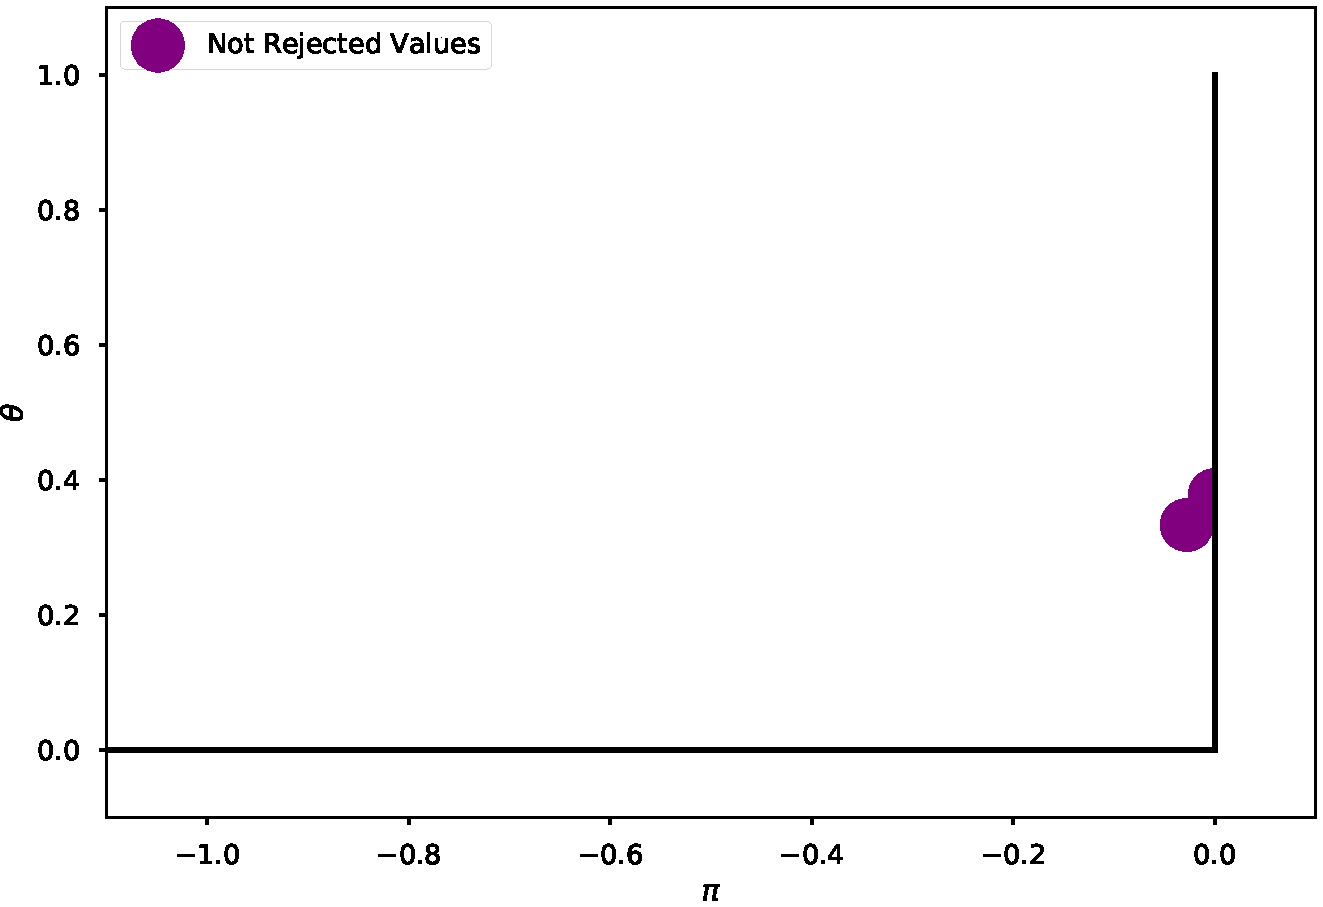
\includegraphics[width=.5\textwidth]{confidence_region_2.pdf}
    \end{figure}

\end{frame}

\section{Conclusion}

\begin{frame}[c]{Conclusion}

  \begin{enumerate}
%
      \item[\cmark] The model.
      \bigskip
%
  \item[\cmark] Asymptotic results for the reduced-form and structural parameters.
      \bigskip
%
  \item[\cmark] Confidential inference algorithm for minimum distance estimation and accompanying theory. 
      \bigskip
%
    \item[\cmark] Simulation results. 
      \bigskip
%
    \item[\cmark] Empirical results using data on the S\&P 500.
%
  \end{enumerate}

\end{frame}

\end{document}

